% !TeX program = pdflatex

\documentclass[twocolumn]{IECEjournal} % lineno, proof, onecolumn
\usepackage{amsmath}
\usepackage{listings}
\usepackage{xcolor}
\usepackage{color}
\usepackage{caption}
\usepackage{amssymb}
\usepackage[none]{hyphenat}
\usepackage{enumitem}
\usepackage{tikz}
\usetikzlibrary{shapes.geometric, arrows}
\tikzstyle{startstop} = [ellipse, minimum width=2.5cm, minimum height=1cm, text centered, draw=black, fill=red!30]
\tikzstyle{process} = [rectangle, rounded corners, minimum width=2.5cm, minimum height=1cm, text centered, draw=black, fill=blue!30]
\tikzstyle{arrow} = [thick,->,>=stealth]
\usepackage{graphicx}
\usepackage{tikz-cd}
\usepackage{lipsum}
\usepackage{multicol}
\usepackage{float}
\usepackage[ruled]{algorithm2e}
\let\procedure\relax
\let\endprocedure\relax

\renewcommand{\abstractname}{Resumen}
\renewcommand{\keywordsname}{Palabras clave}

\usetikzlibrary{arrows.meta}
\graphicspath{{res/},{media/},{figures/}}

\AtBeginEnvironment{thebibliography}{\small}
\usepackage{newfloat,array}
\newcolumntype{P}[1]{p{#1}<{\raggedright}}
\DeclareFloatingEnvironment[fileext=prc,placement={htb},name=Procedure]{prc}
\captionsetup[prc]{labelfont={sf,bf,normalsize},skip=0pt}
\newcounter{procedure}
\setcounter{procedure}{1}
\NewDocumentEnvironment{procedure}{O{ht} m}{%
\begin{prc}[#1]
\caption{#2}
\begin{mdframed}[%
  backgroundcolor=black!10!white,
  font=\ttfamily,
  roundcorner=2pt]
\end{mdframed}\end{prc}}

\articletype{Research Article}
\submitdate{20/12/2024}
\acceptdate{20/12/2024}
\pubdate{20/12/2024}

\jnlsetup{%
    author  = {Araujo R., Robert, Rivera F., Alexis y Salinas J., Allen},
    journal = {Universidad Nacional Agraria La Molina}, 
    title   = {Clusterización de Nubes Potencialmente Precipitables en Cusco durante el periodo 12/2023 al 04/2024},  % Manuscript title
    ctitle  = {Clusterización de Nubes Potencialmente Precipitables en Cusco durante el periodo 12/2023 al 04/2024},  % Manuscript title
    volume  = {1},
    number  = {1},
    year    = {2024},    
}
% Data availability
\dataavail{%
The data used to support the findings of this study are available from the corresponding author upon request.}

\setcounter{page}{1}
\makeatother
\begin{document}

\author[1]{Araujo R., Robert}
\author[2]{Rivera F., Alexis}
\author[3]{Salinas J., Allen}

\affil[1]{Universidad Nacional Agraria La Molina, Lima - Perú / 20221343@lamolina.edu.pe}
\affil[2]{Universidad Nacional Agraria La Molina, Lima - Perú / 20221348@lamolina.edu.pe}
\affil[3]{Universidad Nacional Agraria La Molina, Lima - Perú / 20221349@lamolina.edu.pe}

\ifproof
\input{proof}
\fi

\maketitle

\abstract{El análisis de datos satelitales permite comprender fenómenos meteorológicos complejos. En este estudio se empleó el algoritmo K-means en datos de temperatura de brillo de la banda 13 del satélite GOES-16 para identificar patrones de nubes potencialmente precipitables sobre Cusco entre diciembre de 2023 y abril de 2024. Tras preprocesar los datos y determinar el número óptimo de clusters mediante el método del codo, se utilizó el valor de K como 4. Por otra parte, se identificaron agrupaciones basadas en temperaturas de brillo. Estas se compararon con datos de precipitación del SENAMHI de 12 estaciones meteorológicas de la zona de estudio, observándose una relación entre temperaturas bajas y precipitaciones.}

\noindent \textbf{Palabras Clave:} k-means, Clustering, Nubes precipitables, Imágenes IR GOES-16, Temperatura de brillo, Cusco.
%% -- citationblock
\citationblock

\section{Introducción}
La identificación y análisis de patrones climáticos mediante datos satelitales se ha convertido en una herramienta esencial para comprender fenómenos meteorológicos complejos~\cite{1}. Este trabajo se centra en la clusterización de nubes potencialmente precipitables sobre el territorio del departamento de Cusco, Perú utilizando datos provenientes del satélite GOES-16 de la banda 13, específicamente del canal infrarrojo termal (CMI). Para ello, se emplea el algoritmo de K-means, que permite agrupar píxeles de la imagen satelital según sus características de temperatura de brillo. Dado que el Perú presenta una geografía y clima altamente variables~\cite{2}, la delimitación de las áreas de estudio y la preprocesamiento de los datos, incluyendo la filtración de valores faltantes y el ajuste de coordenadas, son pasos clave para asegurar resultados precisos. Este enfoque no solo facilita el estudio de patrones nubosos relacionados con precipitaciones, sino que también puede aportar al monitoreo y predicción de eventos climáticos adversos en una región particularmente vulnerable a los efectos del cambio climático.

\section{Antecedentes}
En la investigación de Yuchechen et al.~\cite{3}, se implementó el algoritmo de agrupamiento no supervisado k-means/k-means++ en imágenes diarias de anomalías estandarizadas de temperatura de brillo derivados de los datos infrarrojos del Satélite Ambiental Operacional Geoestacionario (GOES)-13 para el período del 1 de diciembre de 2010 al 30 de noviembre de 2016 para la región de Sudamérica, con el fin de clasificar nubes de diferentes características. Se obtuvo 4 grupos que se ordenaron por su valor medio de temperatura de brillo, de modo que cuanto menor sea el orden de los grupos, más desarrollo vertical tienen las nubes que representan. Por otro lado, en Shan Zeng et al.~\cite{4}se empleó análisis de clusters fuzzy k-means (FKM) a un subconjunto de los parámetros reportados en los productos de datos de CALIPSO lidar de nivel 2 con el objetivo de clasificar las capas detectadas como nubes o aerosoles. Por un lado, FKM es un algoritmo de aprendizaje no supervisado, mientras que el algoritmo CAD operativo de CALIPSO (COCA) es supervisado. Según sus análisis estadísticos muestran que las clasificaciones FKM coinciden con las clasificaciones COCA en más del 94\% de los casos en la troposfera. En general, las incertidumbres de clasificación FKM como las COCA se vieron mínimamente afectadas por el ruido en las mediciones de CALIPSO.

\section{Objetivos}
\subsection{Objetivo General}
Aplicar técnicas de clusterización a datos satelitales de temperatura de brillo de la banda 13 del GOES-16 para identificar y analizar patrones de nubes potencialmente precipitables sobre el departamento de Cusco durante el periodo 12/2023 al 04/2024.

\subsection{Objetivos Específicos}
\begin{itemize}
    \item Determinar el número de K óptimo mediante el método del codo para clusterizar los datos de temperatura de brillo.
    \item Comparar los clusters obtenidos con datos de precipitación de estaciones meteorológicas del SENAMHI dentro del departamento de Cusco.
\end{itemize}

\section{Marco Teórico}
\subsection{Banda 13 IR (Onda Larga Limpia)}
La banda de ventana infrarroja limpia de 10,3 $\mu$m tiene una resolución de 2km y está disponible todo el día. Es menos sensible que otras bandas de ventana infrarroja a la absorción de vapor de agua, lo que mejora las correcciones de humedad atmosférica, ayuda en la clasificación de nubes y otras características atmosféricas, estimación de la temperatura de brillo de la parte superior de las nubes y el tamaño de partícula de las nubes, y caracterización de las propiedades de la superficie en productos derivados.
En esta longitud de onda, la atmósfera es transparente a la radiación, lo que significa que una gran parte de ella logra escapar hacia el espacio exterior sin ser absorbida por los gases atmosféricos~\cite{5}.

\subsection{Precipitaciones Convectivas}
Este tipo de precipitación tiene su origen en la inestabilidad de una masa de  aire más caliente que el circundante, este aire más caliente, asciende y se enfría  adiabáticamente y alcanza su punto de condensación debido a la velocidad vertical adquirida, formándose nubosidad de tipo cumulonimbo, la cual genera  precipitaciones en forma de aguaceros (gran cantidad de agua y gran velocidad de caída)~\cite{6}.
\subsection{Precipitaciones Orográficas}
Cuando los vientos cargados de humedad moviéndose ordinariamente del 
océano a tierra, encuentran una barrera montañosa, la masa de aire es forzada a  ascender, enfriándose y originándose las precipitaciones que se presentan en forma  de lluvia o nieve, siendo muy irregulares en importancia y localización~\cite{6}.


\begin{table}[h]
    \centering    
    \caption{Género, abreviaciòn y altura  en la atmósfera de las nubes.} \label{tab1}
    \scriptsize % Reduce el tamaño del texto dentro de la tabla
    \resizebox{0.5\textwidth}{!}{% Reduce el ancho total al 50% de la página
    \begin{tabular}{lccl}
        \toprule
        \textbf{Género} & \textbf{Abreviación} & \textbf{Altura en la atmósfera} \\ 
        \midrule
        Cirrus & Ci & Alta \\
        Cirrocumulus & Cc & Alta \\
        Cirrostratus & Cs & Alta \\
        Altocumulus & Ac & Media \\
        Altostratus & As & Media \\
        Nimbustratus & Ns & Baja \\
        Stratus & St & Baja \\
        Cumulus & Cu & Nubes convectivas \\
        Cumulonimbus & Cb & Nubes convectivas \\      
        \bottomrule
        
    \end{tabular}%
    }
\end{table}
\scriptsize \textbf{Fuente:} Adaptado de la WMO (World Meteorological Organization) e Iribarne J.V. (1980), citado por Romero~\cite{7}.\\
\normalsize
\subsection{GOES}
El satélite GOES, por sus siglas (Geostationary Operational 
Environmental Satellite), es un  satélite meteorológico y una de las claves de programa estadounidense de la NOAA (National Oceanic and Atmosferic Administration). Los datos obtenidos tanto de imágenes y de sonda del GOES, son continuos y proveen informaciones necesaria para obtener el pronóstico del tiempo, el seguimiento de tormentas severas y para investigaciones en meteorología. Estos satélites operan en órbita geoestacionaria, es decir que orbitan en el plano ecuatorial con la velocidad de rotación de la Tierra. Por lo 
tanto, observan siempre la misma región sobre la superficie, desde una altura de unos 35.800 km, permitiendo la visión completa de un disco sobre la tierra~\cite{6}.

\subsection{Clustering}
El Clustering es un algoritmo que divide un conjunto de objetos de datos en subconjuntos. Cada subconjunto es un grupo, compuesto por objetos con características similares entre sí, pero diferentes a los objetos de otros grupos. El conjunto de grupos resultante de un análisis de grupos se puede denominar cluster. En este contexto, distintos métodos de agrupamiento pueden generar diferentes clusters en el mismo conjunto de datos. Este proceso no es realizado por humanos, sino por el algoritmo de Clustering~\cite{8}.

\section{Metodología}

\begin{figure}[H]
    \centering
    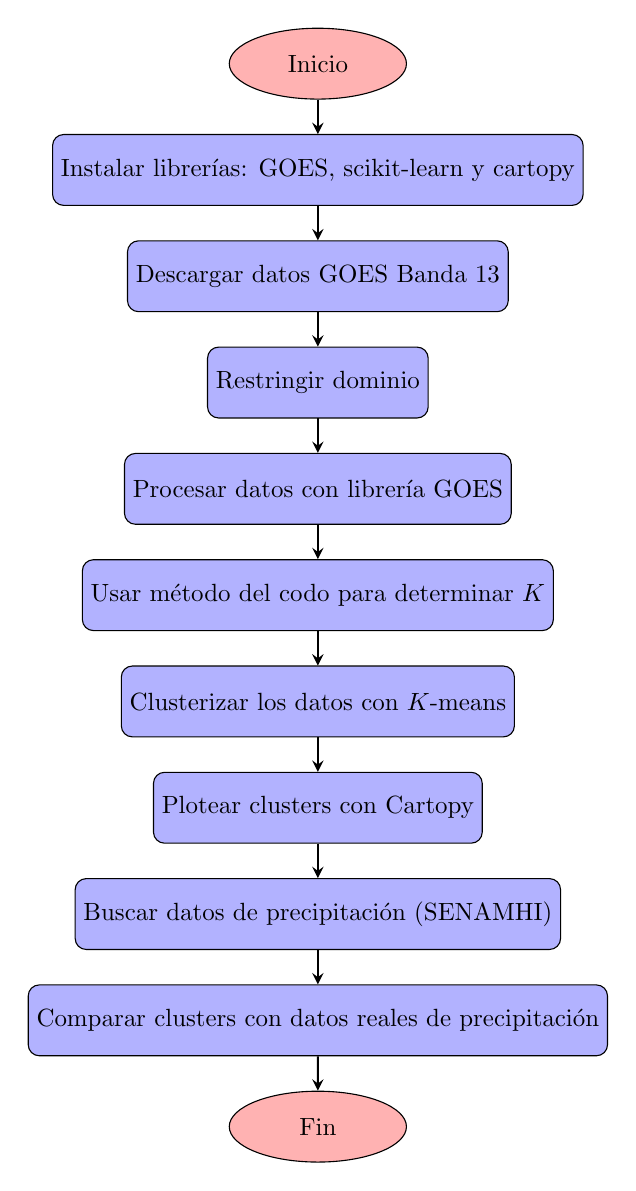
\begin{tikzpicture}[node distance=1.5cm, auto, scale=0.9, every node/.style={scale=0.9}]

        % Nodos del flujograma
        \node (start) [startstop] {Inicio};
        \node (step1) [process, below of=start] {Instalar librerías: GOES, scikit-learn y cartopy};
        \node (step2) [process, below of=step1] {Descargar datos GOES Banda 13};
        \node (step3) [process, below of=step2] {Restringir dominio};
        \node (step4) [process, below of=step3] {Procesar datos con librería GOES};
        \node (step5) [process, below of=step4] {Usar método del codo para determinar $K$};
        \node (step6) [process, below of=step5] {Clusterizar los datos con $K$-means};
        \node (step7) [process, below of=step6] {Plotear clusters con Cartopy};
        \node (step8) [process, below of=step7] {Buscar datos de precipitación (SENAMHI)};
        \node (step9) [process, below of=step8] {Comparar clusters con datos reales de precipitación};
        \node (stop) [startstop, below of=step9] {Fin};

        % Conexiones entre nodos
        \draw [arrow] (start) -- (step1);
        \draw [arrow] (step1) -- (step2);
        \draw [arrow] (step2) -- (step3);
        \draw [arrow] (step3) -- (step4);
        \draw [arrow] (step4) -- (step5);
        \draw [arrow] (step5) -- (step6);
        \draw [arrow] (step6) -- (step7);
        \draw [arrow] (step7) -- (step8);
        \draw [arrow] (step8) -- (step9);
        \draw [arrow] (step9) -- (stop);

    \end{tikzpicture}
    \caption{Flujograma del proceso metodológico.}
    \label{fig1}
\end{figure}

\subsection{Zona de Estudio}
La zona de estudio es el departamento Cusco, ubicado en la región andina de Perú.

\begin{figure}[H]
	\centering
	\includegraphics[width=.90\linewidth]{figures/Resultados/cusco.png}
	\caption{Mapa de Ubicación del departamento Cusco en Perú}
	\label{fig2}
\end{figure}

\subsection{Software}
\begin{itemize}
    \item \textbf{Lenguaje de programación:} Python.
    \item \textbf{Librerías en Python:} GOES para instalar y manejar datos GOES, scikit-learn para aplicar el algoritmo K-means y Cartopy para visualización de los resultados.
\end{itemize}

\subsection{Datos de Imágenes GOES}
Imágenes del canal infrarrojo termal (CMI) del satélite GOES-16 de la banda 13, descargadas en formato .nc (NetCDF) con resolución espacial de aproximadamente 2 km. Para realizar el clustering del periodo de 12/2023 al 04/2024 tomamos datos de algunas horas para simplificar la investigación.

\begin{table}[h]
    \centering
    \caption{Fecha y hora de los datos GOES para cada mes dentro del periodo 12/2023 al 04/2024} \label{tab2}
    \scriptsize % Reduce el tamaño del texto dentro de la tabla
    \resizebox{0.5\textwidth}{!}{% Reduce el ancho total al 60% de la página
    \begin{tabular}{lcccl}
        \toprule
        \textbf{12/2023} & \textbf{01/2024} & \textbf{02/2024} & \textbf{03/2024} & \textbf{03/2024} \\ 
        \midrule
        08/12/2023 (22:30 UTC) & 24/01/2024 (05:30 UTC) & 10/02/2024 (05:30 UTC) & 09/03/2024 (20:30 UTC) & 13/04/2024 (05:30 UTC) \\ 
        29/12/2023 (20:30 UTC) &  & 19/02/2024 (20:30 UTC) & 16/03/2024 (20:30 UTC) &  \\ 
         &  &  & 17/03/2024 (09:00 horas UTC) & \\        
        \bottomrule
        
    \end{tabular}%
    }
\end{table}

\subsection{Algoritmo K-means}
Luego de procesar los datos GOES consideramos asignar a \textbf{K} con el valor de 4 tomando como criterio el método del codo aplicado a nuestros datos. En la Fig (\ref{fig3}) se puede visualizar a partir del cluster 4 la variación la diferencia de las distancias comienza a tener una tiende a dejar ser significativa en los siguientes números de cluster. 

\begin{figure}[H]
	\centering
	\includegraphics[width=.90\linewidth]{figures/codo1.png}
	\caption{Método del codo para varios valores de K}
	\label{fig3}
\end{figure}

\subsection{Datos de Precipitación}
Para los datos de precipitación real, se buscó información de Estaciones Meteorológicas del SENAMHI. En total se eligieron 12 estaciones dentro de la zona de estudio.

\begin{table}[h]
    \centering
    \caption{Estaciones Meteorológicas en la región de estudio.} \label{tab3}
    \scriptsize % Reduce el tamaño del texto dentro de la tabla
    \resizebox{0.5\textwidth}{!}{% Reduce el ancho total al 60% de la página
    \begin{tabular}{lcccl}
        \toprule
        \textbf{Nombre} & \textbf{Latitud} & \textbf{Longitud} & \textbf{Altura (m)} & \textbf{Tipo} \\ 
        \midrule
        Quincemil & 13°13'44.15''S & 70°45'15.84''W & 651 & Convencional \\ 
        Chacllabamba & 13°6'30.77''S & 71°43'12.01''W & 2699 & Convencional \\ 
        Chontachaca & 13°1'26''S & 71°28'4''W & 872 & Convencional \\ 
        Colquepata & 13°21'47.27''S & 71°40'24.1''W & 3696 & Convencional \\ 
        Sibinacocha & 13°55'19.7''S & 71°1'5.63''W & 4880 & Automática \\ 
        Caicay & 13°35'59.96''S & 71°42'1''W & 3117 & Convencional \\ 
        Calca & 13°19'59.97''S & 71°57'18.85''W & 2921 & Automática \\ 
        Urubamba & 13°18'18.6''S & 72°7'28.4''W & 2850 & Convencional \\ 
        Anta Ancachuro & 13°28'20.71''S & 72°13'7.54''W & 3324 & Convencional \\
        Sicuani & 14°14'14.5''S & 71°14'12.1''W & 3534 & Automática \\
        Aymaña & 13°52'22.03''S & 70°40'3.34''W & 4175 & Automática \\
        Pichari & 12°31'19.9''S & 73°50'22.28''W & 570 & Automática \\       
        \bottomrule
        
    \end{tabular}%
    }
\end{table}
\scriptsize \textbf{Fuente:} Adaptado de SENAMHI (2024). \textit{Datos Hidrometeorológicos a nivel nacional}.\\
Recuperado de \url{https://www.senamhi.gob.pe/?&p=estaciones}
\normalsize

\section{Resultados}
En este apartado se presentan los resultados obtenidos al aplicar técnicas de clusterización a datos satelitales del GOES-16, con el objetivo de identificar y analizar patrones de nubes potencialmente precipitables sobre el territorio de Cusco durante el periodo de diciembre de 2023 a abril de 2024. Estas técnicas permitieron agrupar los datos de temperatura de brillo en rangos asociados a diferentes probabilidades de precipitación, proporcionando una caracterización más detallada de las condiciones atmosféricas en la región.

\begin{figure}[H]
	\centering
	\includegraphics[width=.90\linewidth]{figures/Resultados/resultado1a.png}
	\caption{Mapa de temperatura de brillo para el 08/12/2023 a las 22:30 horas UTC}
	\label{fig4}
\end{figure}

\begin{figure}[H]
	\centering
	\includegraphics[width=.90\linewidth]{figures/Resultados/resultado1b.png}
	\caption{Mapa de clusters para el 08/12/2023 a las 22:30 horas UTC}
	\label{fig5}
\end{figure}

\begin{table}[h!]
    \centering
    \label{tab4}
    \begin{tabular}{|c|c|}
    \hline
    \textbf{Cluster} & \textbf{Valor} \\
    \hline
    Cluster 3 & 207.46 \\
    Cluster 0 & 230.76 \\
    Cluster 2 & 258.65 \\
    Cluster 1 & 281.75 \\
    \hline
    \end{tabular}
    \caption{Media de cada cluster para el 08/12/2023 a las 22:30 horas UTC}
\end{table}

\begin{figure}[H]
	\centering
	\includegraphics[width=.90\linewidth]{figures/Resultados/resultado2a.png}
	\caption{Mapa de temperatura de brillo para el 29/12/2023 a las 20:30 horas UTC}
	\label{fig6}
\end{figure}

\begin{figure}[H]
	\centering
	\includegraphics[width=.90\linewidth]{figures/Resultados/resultado2b.png}
	\caption{Mapa de clusters para el 29/12/2023 a las 20:30 horas UTC}
	\label{fig7}
\end{figure}

\begin{table}[h!]
    \centering
    \label{tab5}
    \begin{tabular}{|c|c|}
    \hline
    \textbf{Cluster} & \textbf{Valor} \\
    \hline
    Cluster 3 & 218.00 \\
    Cluster 0 & 236.89 \\
    Cluster 2 & 261.33 \\
    Cluster 1 & 286.79 \\
    \hline
    \end{tabular}
    \caption{Media de cada cluster para el 29/12/2023 a las 20:30 horas UTC}
\end{table}

\begin{figure}[H]
	\centering
	\includegraphics[width=.90\linewidth]{figures/Resultados/resultado3a.png}
	\caption{Mapa de temperatura de brillo para el 24/01/2024 a las 05:30 horas UTC}
	\label{fig8}
\end{figure}


\begin{figure}[H]
	\centering
	\includegraphics[width=.90\linewidth]{figures/Resultados/resultado3b.png}
	\caption{Mapa de clusters para el 24/01/2024 a las 05:30 horas UTC}
	\label{fig9}
\end{figure}

\begin{table}[h!]
    \centering
    \label{tab6}
    \begin{tabular}{|c|c|}
    \hline
    \textbf{Cluster} & \textbf{Valor} \\
    \hline
    Cluster 3 & 220.71 \\
    Cluster 0 & 239.48 \\
    Cluster 2 & 262.60 \\
    Cluster 1 & 283.10 \\
    \hline
    \end{tabular}
    \caption{Media de cada cluster para el 24/01/2024 a las 05:30 horas UTC}
\end{table}

\begin{figure}[H]
	\centering
	\includegraphics[width=.90\linewidth]{figures/Resultados/resultado8a.png}
	\caption{Mapa de temperatura de brillo para el 10/02/2024 a las 05:30 horas UTC}
	\label{fig10}
\end{figure}

\begin{figure}[H]
	\centering
	\includegraphics[width=.90\linewidth]{figures/Resultados/resultado8b.png}
	\caption{Mapa de clusters para el 10/02/2024 a las 05:30 horas UTC}
	\label{fig11}
\end{figure}

\begin{table}[h!]
    \centering
    \label{tab7}
    \begin{tabular}{|c|c|}
    \hline
    \textbf{Cluster} & \textbf{Valor} \\
    \hline
    Cluster 0 & 211.34 \\
    Cluster 2 & 235.53 \\
    Cluster 3 & 267.62 \\
    Cluster 1 & 285.10 \\
    \hline
    \end{tabular}
    \caption{Media de cada cluster para el 10/02/2024 a las 05:30 horas UTC}
\end{table}

\begin{figure}[H]
	\centering
	\includegraphics[width=.90\linewidth]{figures/Resultados/resultado4a.png}
	\caption{Mapa de temperatura de brillo para el 19/02/2024 a las 20:30 horas UTC}
	\label{fig12}
\end{figure}

\begin{figure}[H]
	\centering
	\includegraphics[width=.90\linewidth]{figures/Resultados/resultado4b.png}
	\caption{Mapa de clusters para el 19/02/2024 a las 20:30 horas UTC}
	\label{fig13}
\end{figure}

\begin{table}[h!]
    \centering
    \label{tab8}
    \begin{tabular}{|c|c|}
    \hline
    \textbf{Cluster} & \textbf{Valor} \\
    \hline
    Cluster 2 & 218.07 \\
    Cluster 0 & 238.71 \\
    Cluster 3 & 263.29 \\
    Cluster 1 & 288.73 \\
    \hline
    \end{tabular}
    \caption{Media de cada cluster para el 19/02/2024 a las 20:30 horas UTC}
\end{table}

\begin{figure}[H]
	\centering
	\includegraphics[width=.90\linewidth]{figures/Resultados/resultado5a.png}
	\caption{Mapa de temperatura de brillo para el 09/03/2024 a las 20:30 horas UTC}
	\label{fig14}
\end{figure}

\begin{figure}[H]
	\centering
	\includegraphics[width=.90\linewidth]{figures/Resultados/resultado5b.png}
	\caption{Mapa de clusters para el 09/03/2024 a las 20:30 horas UTC}
	\label{fig15}
\end{figure}

\begin{table}[h!]
    \centering
    \label{tab9}
    \begin{tabular}{|c|c|}
    \hline
    \textbf{Cluster} & \textbf{Valor} \\
    \hline
    Cluster 3 & 216.24 \\
    Cluster 1 & 238.21 \\
    Cluster 2 & 266.79 \\
    Cluster 0 & 290.67 \\
    \hline
    \end{tabular}
    \caption{Media de cada cluster para el 09/03/2024 a las 20:30 horas UTC}
\end{table}

\begin{figure}[H]
	\centering
	\includegraphics[width=.90\linewidth]{figures/Resultados/resultado6a.png}
	\caption{Mapa de temperatura de brillo para el 16/03/2024 a las 20:30 horas UTC}
	\label{fig16}
\end{figure}

\begin{figure}[H]
	\centering
	\includegraphics[width=.90\linewidth]{figures/Resultados/resultado6b.png}
	\caption{Mapa de clusters para el 16/03/2024 a las 20:30 horas UTC}
	\label{fig17}
\end{figure}

\begin{table}[h!]
    \centering
    \label{tab10}
    \begin{tabular}{|c|c|}
    \hline
    \textbf{Cluster} & \textbf{Valor} \\
    \hline
    Cluster 3 & 222.25 \\
    Cluster 1 & 248.00 \\
    Cluster 0 & 272.26 \\
    Cluster 2 & 291.12 \\
    \hline
    \end{tabular}
    \caption{Media de cada cluster para el 16/03/2024 a las 20:30 horas UTC}
\end{table}


\begin{figure}[H]
	\centering
	\includegraphics[width=.90\linewidth]{figures/Resultados/resultado9a.png}
	\caption{Mapa de temperatura de brillo para el 17/03/2024 a las 09:00 horas UTC}
	\label{fig18}
\end{figure}

\begin{figure}[H]
	\centering
	\includegraphics[width=.90\linewidth]{figures/Resultados/resultado9b.png}
	\caption{Mapa de clusters para el 17/03/2024 a las 09:00 horas UTC}
	\label{fig19}
\end{figure}

\begin{table}[h!]
    \centering
    \label{tab11}
    \begin{tabular}{|c|c|}
    \hline
    \textbf{Cluster} & \textbf{Valor} \\
    \hline
    Cluster 2 & 222.51 \\
    Cluster 0 & 248.96 \\
    Cluster 3 & 262.08 \\
    Cluster 1 & 278.71 \\
    \hline
    \end{tabular}
    \caption{Media de cada cluster para el 17/03/2024 a las 09:00 horas UTC}
\end{table}

\begin{figure}[H]
	\centering
	\includegraphics[width=.90\linewidth]{figures/Resultados/resultado7a.png}
	\caption{Mapa de temperatura de brillo para el 13/04/2024 a las 05:30 horas UTC}
	\label{fig20}
\end{figure}

\begin{figure}[H]
	\centering
	\includegraphics[width=.90\linewidth]{figures/Resultados/resultado7b.png}
	\caption{Mapa de clusters para el 13/04/2024 a las 05:30 horas UTC}
	\label{fig21}
\end{figure}

\begin{table}[h!]
    \centering
    \label{tab12}
    \begin{tabular}{|c|c|}
    \hline
    \textbf{Cluster} & \textbf{Valor} \\
    \hline
    Cluster 1 & 210.54 \\
    Cluster 2 & 256.87 \\
    Cluster 3 & 272.23 \\
    Cluster 0 & 284.47 \\
    \hline
    \end{tabular}
    \caption{Media de cada cluster para el 13/04/2024 a las 05:30 horas UTC}
\end{table}


A continuación se presentará un resumen de las precipitaciones medidas en las Estaciones Meteorológicas ubicadas en la zona de estudio (\ref{tab1}).

\begin{table}[h]
    \centering
    \caption{Intensidad de las Precipitaciones en las Estaciones Convencionales Meteorológicas.} \label{tab13}
    \scriptsize % Reduce el tamaño del texto dentro de la tabla
    \resizebox{0.5\textwidth}{!}{% Reduce el ancho total al 50% de la página
    \begin{tabular}{lcccl}
        \toprule
        \textbf{Nombre} & \textbf{Fecha} & \textbf{Precipitación (mm)} \\ 
        \midrule
        Quincemil & 08/12/23 & 99.6 \\ 
        Urubamba & 08/12/23 & 20.7 \\ 
        Chacllabamba & 08/12/23 & 36.5 \\
        Caicay & 08/12/23 & 15.0 \\
        Chontachaca & 29/12/23 & 60.6 \\
        Quincemil & 24/01/24 & 121.4 \\
        Quincemil & 19/02/24 & 109.9 \\
        Anta Ancachuro & 19/02/24 & 8.0 \\
        Quincemil & 09/03/24 & 63.6 \\
        Chontachaca & 16/03/24 & 47.6 \\
        Colquepata & 16/03/24 & 22.8 \\
        Urubamba & 16/03/24 & 15.0 \\
        Anta Ancachuro & 16/03/24 & 8.2 \\
        Quincemil & 13/04/24 & 12.6 \\  
        \bottomrule
        
    \end{tabular}%
    }
\end{table}

\begin{table}[h]
    \centering    
    \caption{Intensidad de las Precipitaciones en las Estaciones Automáticas Meteorológicas.} \label{tab14}
    \scriptsize % Reduce el tamaño del texto dentro de la tabla
    \resizebox{0.5\textwidth}{!}{% Reduce el ancho total al 50% de la página
    \begin{tabular}{lcccl}
        \toprule
        \textbf{Nombre} & \textbf{Fecha} & \textbf{Horas} & \textbf{Precipitación (mm)} \\ 
        \midrule
        Aymaña & 08/12/23 & 21-23 & 6.0 \\
        Sibinacocha & 29/12/23 & 20-23 & 3.7 \\
        Sibinacocha & 24/01/24 & 04-08 & 1.7 \\
        Calca & 24/01/24 & 02-06 & 15.6 \\
        Sicuani & 24/01/24 & 00-06 & 12.0 \\
        Aymaña & 24/01/24 & 01-05 & 13.1 \\
        Sibinacocha & 10/02/24 & 11-12 & 13.8 \\
        Calca & 10/02/24 & 02-06 & 9.8 \\        
        Aymaña & 09/03/24 & 15-16 & 15.2 \\
        Pichari & 17/03/24 & 04-08 & 96.6 \\       
        \bottomrule
        
    \end{tabular}%
    }
\end{table}

\section{Discusiones}

Se realizaron análisis comparativos entre los clusters obtenidos y los datos de precipitación registrados por las estaciones meteorológicas del SENAMHI, presentados en la las tablas (\ref{tab13}) y (\ref{tab14}). Estos análisis tuvieron como objetivo validar la correspondencia entre los patrones satelitales, como la temperatura de brillo representado por los clusters, y las mediciones in situ.

Para la primera fecha, 08/12/24, tanto en el mapa de los clusters (\ref{fig5}) como en el mapa de la temperatura de brillo (\ref{fig4}), se observa en el suroeste de ambos mapas una temperatura de brillo baja. Esto coincide con los datos de la tabla (\ref{tab13}), donde la estación Quincemil (E. Convencional), ubicada en el suroeste de la región de Cusco, registró un valor de precipitación extremadamente alto (99.6 mm). Otras estaciones al centro-oeste de la región también reportaron precipitaciones moderadamente altas: Urubamba (E. Convencional) con 20.7 mm, Chacllabamba (E. Convencional) con 36.5 mm, y Caicay (E. Convencional) con 15 mm. En el caso de Aymaña (E. Automática), se registraron 6 mm de precipitación acumulada entre las 21 y 23 horas.

En la segunda fecha, 29/12/23, los mapas (\ref{fig6}) y (\ref{fig7}) muestran temperaturas de brillo bajas en el sur, noreste y centro de la región. Según la tabla (\ref{tab13}), Chontachaca (E. Convencional), ubicada en el centro de la región, registró una precipitación significativa de 60.6 mm. Por su parte, Sibinacocha (E. Automática), localizada en el sur, reportó 3.7 mm de precipitación acumulada entre las 20 y 23 horas.

En el mes de enero, para la única fecha de muestreo, 24/01/24, el mapa de temperatura de brillo (\ref{fig8}) muestra niveles bajos en toda la región sur, representados claramente por el cluster 3 (\ref{fig9}), el cual tiene las temperaturas más bajas (\ref{tab5}). En esta zona afectada, la estación Quincemil (E. Convencional) registró precipitaciones extremadamente altas de 121.4 mm. Además, las estaciones automáticas de Sibinacocha (1.7 mm), Calca (15.6 mm), Sicuani (12.0 mm) y Aymaña (13.1 mm) registraron precipitaciones durante las horas de madrugada.

En febrero, hubo dos fechas de muestreo: 10/02/24 y 19/02/24. Para la primera fecha, el mapa (\ref{fig10}) muestra temperaturas de brillo bajas en gran parte de la región, asociadas al cluster 0 (\ref{fig11}), que representa las temperaturas más bajas (\ref{tab6}). En esta zona, la estación Sibinacocha (E. Automática) registró 13.8 mm de precipitación entre las 11 y 12 horas. En la segunda fecha, los mapas (\ref{fig12}) y (\ref{fig13}) destacan temperaturas bajas en gran parte del territorio. En esta ocasión, Quincemil (E. Convencional) y Anta Ancachuro (E. Convencional) registraron precipitaciones de 109.9 mm y 8.0 mm, respectivamente.

En marzo, las fechas de muestreo fueron 09/03/24, 16/03/24 y 17/03/24. Para la primera fecha, los mapas (\ref{fig14}) y (\ref{fig15}) muestran temperaturas de brillo bajas en el centro y sur de la región. En estas áreas, Quincemil (E. Convencional) reportó 63.6 mm de precipitación, mientras que Aymaña (E. Automática) registró 15.2 mm entre las 15 y 16 horas. En la segunda fecha, los mapas (\ref{fig16}) y (\ref{fig17}) evidencian bajas temperaturas de brillo en el centro, oeste y sur. Las estaciones afectadas fueron Chontachaca (E. Convencional) con 47.6 mm, Colquepata (E. Convencional) con 22.8 mm, Urubamba (E. Convencional) con 15.0 mm, y Anta Ancachuro (E. Convencional) con 8.2 mm.

Finalmente, en abril, para la fecha 13/04/24, los mapas (\ref{fig20}) y (\ref{fig21}) muestran que la principal zona afectada es el suroeste de la región. En esta área, la estación Quincemil (E. Convencional) registró una precipitación de 12.6 mm.

Los resultados mencionados respaldan, en términos generales, la hipótesis de que los datos satelitales pueden ser utilizados eficazmente para identificar patrones de nubes precipitables.

Aunque los resultados fueron consistentes con las expectativas, no se alcanzó una precisión del 100\%. Esta discrepancia podría atribuirse a varias limitaciones, como la resolución espacial y temporal de los datos satelitales, la influencia de condiciones atmosféricas locales no detectadas por los sensores del GOES-16 y la naturaleza probabilística inherente a los métodos de clusterización, que introduce cierto grado de incertidumbre en la clasificación.

Por lo tanto, es importante destacar la necesidad de realizar un monitoreo continuo de las temperaturas de brillo y los clusters, ya que las regiones con temperaturas bajas pueden variar con el tiempo, afectando a diferentes provincias y alterando los registros de precipitación en otras zonas de la región de estudio.

Los valores positivos reportados en las tablas refuerzan la utilidad de los clusters para identificar eventos precipitables. Sin embargo, estos hallazgos también subrayan la necesidad de integrar fuentes de datos adicionales y realizar ajustes en los algoritmos empleados. Estos ajustes podrían incluir validación cruzada con datos de estaciones meteorológicas y modelos de pronóstico meteorológico, con el objetivo de mejorar la confiabilidad y precisión de los resultados obtenidos.

\section{Conclusiones}
Las técnicas de clusterización aplicadas en los datos de temperatura de brillo de la banda 13 del GOES-16 permiten identificar patrones de nubes asociadas con precipitaciones en Cusco durante el periodo 12/2023 al 04/2024. De forma específica se concluyó en lo siguiente:

\begin{itemize}
      \item  Se registró en los mapas de temperatura de brillo un patrón bastante similar con los mapas de clusters para cada fecha, por lo que el número de clusters como 4 fue óptimo.
      \item  La comparación con los datos de precipitación de las 12 estaciones meteorológicas seleccionadas del SENAMHI coinciden en su mayoría con los valores visualizados de los clusters en la zona de Cusco para las horas seleccionadas.
      
\end{itemize}

\section*{Conflictos de interés}
Los autores declaran no tener conflictos de interés.

\section*{Agradecimientos}
Este trabajo fue apoyado sin ningún financiamiento.

%\bibliography{sample,citation}
%\printbibliography[notcategory=fullcited,resetnumbers=true]

\begin{fullwidth}
\renewcommand{\bibname}{Referencias}
\begin{thebibliography}{99}
\bibitem{1} Gaibor Velasco, N. I., López Bravo, O. E., Vallejo Ilijama, M. T., \& Arreguín Samano, M. (2023). Análisis de la variabilidad climática utilizando producto satelital MERRA 2 para la microcuenca del Rio Chazo Juan-Bolívar Ecuador (pp. 98-99). [\href{https://doi.org/10.5281/zenodo.7930679}{CrossRef}]

\bibitem{2} Llacza, A., Acuña, D., Jácome, G., De la Cruz, G., Paredes, J., Bruno, J., Alvarez, E., Flores, W., Urdanivia, F., \& Sulca, B. (2021). Escenarios climáticos al 2050 en el Perú: Cambios en el clima promedio. Lima: Servicio Nacional de Meteorología e Hidrología del Perú (p. 8). [\href{https://hdl.handle.net/20.500.12542/1470}{CrossRef}]

%Está cita está correcta
\bibitem{3} Yuchechen, A. E., Lakkis, S. G., Caferri, A., Canziani, P. O., \& Muszkats, J. P. (2020). A Cluster Approach to Cloud Cover Classification over South America and Adjacent Oceans Using a k-means/k-means++ Unsupervised Algorithm on GOES IR Imagery. Remote Sensing, 12(18), 2991 (p. 1).[\href{https://doi.org/10.3390/rs12182991}{CrossRef}]

\bibitem{4} Zeng, S., Vaughan, M., Liu, Z., Trepte, C., Kar, J., Omar, A., Winker, D., Lucker, P., Hu, Y., Getzewich, B., \& Avery, M. (2019). Application of high-dimensional fuzzy k-means cluster analysis to CALIOP/CALIPSO version 4.1 cloud–aerosol discrimination. Atmospheric Measurement Techniques, 12(4), 2261-2285 (p. 1).[\href{https://doi.org/10.5194/amt-12-2261-2019}{CrossRef}]

\bibitem{5} NOAA-NASA. (s.f.). Abi Band 13 (10.3 um) Quick Guide. Obtenido de [\href{http://cimss.ssec.wisc.edu/goes/OCLOFactSheetPDFs/ABIQuickGuide_Band13.pdf}{CrossRef}]

\bibitem{6} Paz, S., Mario, R., \& Diego, L. (2021). Estimación de precipitación mediante el empleo de  imágenes satelitales (pp. 48 y 60). [\href{https://hdl.handle.net/20.500.12542/1470}{CrossRef}]

\bibitem{7} Romero, P. (2022). Estudios sobre clasificación de tipos de nubes en imágenes de satélites meteorológicos usando procesamiento de imágenes y técnicas de aprendizaje automático. Tesis (Lic. en Física)--Universidad Nacional de Córdoba, Facultad de Matemática, Astronomía, Física y Computación (p. 9) [\href{http://hdl.handle.net/11086/24824}{CrossRef}]

\bibitem{8} Han, J., Kamber, M., \& Pei, J.(2012). Data Mining Concepts and Techniques. Third edition (p. 444) [\href{https://doi.org/10.1016/C2009-0-61819-5}{CrossRef}]
\end{thebibliography}
\end{fullwidth}

 % 
\makeatletter
\if@twocolumn

\else

\fi

\makeatother

\end{document}